\documentclass[parskip=half]{scrartcl}
\usepackage{fontspec}
\usepackage[ngerman]{babel}
\usepackage{hyperref}
\usepackage{csquotes}
\usepackage{biblatex}

\bibliography{ausarbeitung}

% nicht einmal notwendig, ist eh standard
%\fontspec{Latin Modern Roman}

\author{Simon~Becker, Marek~Kubica\\TU~München}
\title{Die Geschichte der Rechnerarchitektur\\
Sommersemester 2013\\
Verarbeitung von Lochkarten: Hollerith und die D11}

\date{22.~März~2013}

\hypersetup{
%	bookmarks=true,          % show bookmarks bar?
%	unicode=false,           % non-Latin characters in Acrobat’s bookmarks
%	pdftoolbar=true,         % show Acrobat’s toolbar?
%	pdfmenubar=true,         % show Acrobat’s menu?
%	pdffitwindow=false,      % window fit to page when opened
	pdfstartview={FitH},     % fits the width of the page to the window
	pdftitle={Verarbeitung von Lochkarten: Hollerith und die D11},     % title
	pdfauthor={Simon Becker, Marek Kubica},   % author
	pdfsubject={Seminarausarbeitung}, % subject of the document
%	pdfcreator={Creator},    % creator of the document
%	pdfproducer={Producer},  % producer of the document
	pdfkeywords={d11} {dehomag} {hollerith}, % list of keywords
%	pdfnewwindow=true,       % links in new window
%	colorlinks=true,         % false: boxed links; true: colored links
%	linkcolor=black,         % color of internal links (original: red)
%	linktoc=section          % which part of a toc-entry to link (possible: none, section, page, all)
%	citecolor=black,         % color of links to bibliography (original: green)
%	filecolor=black,         % color of file links (original: magenta)
%	urlcolor=black,          % color of external links (original: cyan)
%	linkbordercolor={1 0 0}, % color of frame around internal links (if colorlinks=false)
%	citebordercolor={0 1 0}, % color of frame around citations (if colorlinks=false)
%	urlbordercolo={0 1 1}    % color of frame around URL links (if colorlinks=false)
}

\begin{document}
\maketitle

\begin{abstract}

Herman Hollerith, ein amerikanischer Erfinder, popularisiert gegen Ende des
19.~Jahrhunderts die mechanische Datenverarbeitung. Dabei setzt er die von
Jaquard bekannte Technik der Lochkarten in einem anderen Kontext um und
revolutioniert sowohl Volkszählungen als auch die Buchhaltung. Wie es zu diesen
Entwicklungen kam, wie Hollerith seine Idee etablieren konnte und auf welche Hindernisse 
er traf, werden im Folgenden beleuchtet.

Ein ausgefeiltes Beispiel des von Hollerith erfundenen Systems ist die in
Deutschland entwickelte Tabelliermaschine D11. Es wird beschrieben wie diese Maschine funktioniert und welche Weiterentwicklungen es gab. 
Des Weiteren wird ein Blick in die politikgeschichtlichen
Zusammenhänge geworfen sowie ein Bogen zur Verwendung von Lochkarten in der
heutigen Zeit gespannt.

\end{abstract}

\section{Einleitung}
\label{sec:einleitung}

Um die von Hollerith geprägte Geschichte der Lochkarten zu verstehen, ist es
zunächst einmal notwendig, den Begriff des Tabellierens zu klären.

Beim Tabellieren werden nicht zwingend vorsortierte Daten nach bestimmten
Kriterien ausgewertet und danach für weitere Verarbeitungen sortiert abgelegt.
Dieser Vorgang ist notwendig um Datensätze nach bestimmten, gegebenfalls sogar
voneinander abhängigen Kriterien auswerten zu können. So kann durch das
Tabellieren von Volkszählungsdatensätzen bestimmt werden, wie viele Einwohner
eines Landes Staatsbürger sind und wie viele Immigranten. Die Immigranten etwa
können daraufhin nach weiteren Kriterien analysiert werden, wie etwa
Ursprungsland oder Einwanderungsjahr.

Solch eine Verarbeitung von Daten ist für Bevölkerungsstatistiken interessant,
kann aber auch verwendet werden um Firmendaten zu verarbeiten, wie etwa die
Arbeitszeiten von Angestellten, die Einnahmen von Kundenverträgen, also
allgemein vieles was unter dem Namen Buchhaltung zu finden ist.

Dabei ist zu beachten, dass das Tabellieren nicht zwingend eine Maschine
vorraussetzt. Vor Holleriths Tabelliermaschinen wurde dieser Vorgang von Hand
ausgeführt und Hollerith hat diese mechanische Tätigkeit automatisiert.

Heutzutage sind Tabelliermaschinen selbst ausgestorben, aber ihre Funktion ist
in Software wie Tabellenkalkulationen und Datenbanken noch bis heute
unverzichtbar.

\section{Herman Hollerith}
\label{sec:hollerith}

Herman Hollerith wurde am 29.~Februar 1860 in Buffalo, New York als
Sohn deutschstämmiger Einwanderer geboren. Dies bedeutet auch, dass Hollerith selbst
US-Amerikaner war, jedoch mit einem deutsch klingenden Namen. Diese
Unterscheidung ist später für die Dehomag wichtig. Holleriths Geschichte spielt sich aber hauptsächlich in den USA ab.

Hollerith studierte Minenbau und erlangte 1879 einen \enquote{Engineer of
Mines}-Abschluss, auf den 1880 sein Ph.D. folgte.

% TODO: heirat
% todo familie

% todo am MIT

1884 arbeitete Hollerith in einem Zensusbüro. Dort kam er mit der Realität von
Volkszählungen und ihrer Auswertung in Kontakt. Damals war der Ablauf von Volkszählungen folgendermaßen: Die Bürger mussten Fragebögen ausfüllen, auf denen eine Reihe von Fakten
abgefragt wurden. Diese Fragebögen wurden später eingesammelt und an zentraler
Stelle, im Zensusbüro, ausgewertet.

Dabei wurden die Datensätze durchgegangen, nach bestimmten Kriterien
ausgewertet und sortiert. Um komplexere Kriterien auszuwerten, mussten die
Datensätze mehrmals durchlaufen werden. Beispiele dafür könnten etwa sein, wie viele
Immigranten selbstständig sind (Auswertung nach Anzahl der Immigranten, danach
diese Daten nach Selbstständigen auswerten) oder wie viele Weiße wurden 1880
geboren (Auswertung nach Hautfarbe und danach nochmals nach Geburtsjahr).

Dieses Verfahren ist effektiv, aber erfordert viel Aufwand die Datensätze
durchzugehen und richtig einzusortieren. Hollerith erkannte, dass diese Arbeit
eine im Grunde mechanische war und dass diese durch Maschinen unterstützt
werden könnte.

Diese Erkenntnis nutzte Hollerith um Maschinen zu bauen, die diese Arbeit
automatisierten. Er gründete eine Firma, auf die später noch näher eingegangen wird. Die Idee wie Hollerith Daten repräsentierte, wird in
\autoref{sec:lochkarten} beschrieben. Die von ihm entwickelten Maschinen werden
in \autoref{sec:1890} sowie \autoref{sec:1900} genauer beleuchtet. Da Hollerith
neben seiner Tätigkeit als Erfinder auch Geschäftsmann war, wird sein
kommerzieller Erfolg in \autoref{sec:commerce} beschrieben.

Nachdem Hollerith seine Firma verkaufte, arbeitete er einige Jahre noch
beratend mit, bevor er sich vollständig mit seiner Familie auf seine gekaufte
Farm zurückzog und dort seine restlichen Jahre in Wohlstand
verbrachte~\cite{austrian1982herman}. Herman Hollerith verstarb am 17.~November
1929.

\subsection{Lochkarten als Datensätze}
\label{sec:lochkarten}

Hollerith suchte nach einer Möglichkeit, die Datensätze zu repräsentieren, als
ihm bei einer Zugfahrt die Idee kam, eine Lochkarte zu verwenden. Inspiriert
wurde er durch sein Zugticket, welches ein \enquote{Punch Photograph} war. Die
Idee hinter einem \enquote{Punch Photograph} war, dass die Eigenschaften des
Ticketbesitzers auf einem Bogen Papier mit Löchern eingestanzt werden, so dass
dieses Ticket nicht mehr ohne Weiteres übertragbar ist. Dabei werden
Eigenschaften wie Geschlecht, ungefähres Aussehen, ungefähres Alter sowie
Strecke und Fahrtzeit durch das Stanzen eines Loches notiert.

Auf diese Weise konnte man die Lochkarte einer Person als einzelnen Datensatz
ansehen, in dem verschiedene Daten über eine Person durch die Anordnung der
Löcher enkodiert werden können. Tatsächlich nutzte Hollerith in der Anfangszeit
eine Handstanze wie sie Fahrkartenkontrolleure eingesetzt haben, so dass die
Löcher sich an dem Rand der Karte befanden.

\subsection{US-Volkszählung 1890}
\label{sec:1890}

Im 19ten Jahrhundert wurde in den USA die Volkszählung alle zehn Jahre durch
das Zensusbüro organisiert und ausgeführt. Für die Durchführung einer solchen
Volkszählung wurde vor der Zählung der aktuelle Stand der Technik evaluiert und
es fand eine Ausschreibung statt. Für die Volkszählung 1890 wurde zu Holleriths
Gunsten Robert P. Porter, ein persönlicher Freund von Hollerith, zum Leiter
erklärt. Porter war ein begeisterter Befürworter der elektrischen
Tabelliermaschinen~\cite{austrian1982herman}.

\begin{figure}[h]
  \centering
  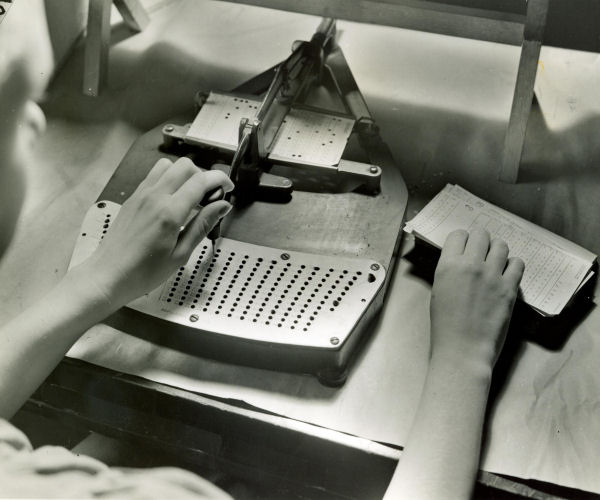
\includegraphics[width=\textwidth]{pantograph}
  \caption{Die \enquote{pantograph punch}, oben die in dieser Abbildung
    bedruckte Lochkarte, unten die Vorlage in die der Hebel abgesenkt wird um
    die Löcher zu stanzen~\cite{pantograph}.}
  \label{fig:pantograph}
\end{figure}

\begin{figure}[h]
  \centering
  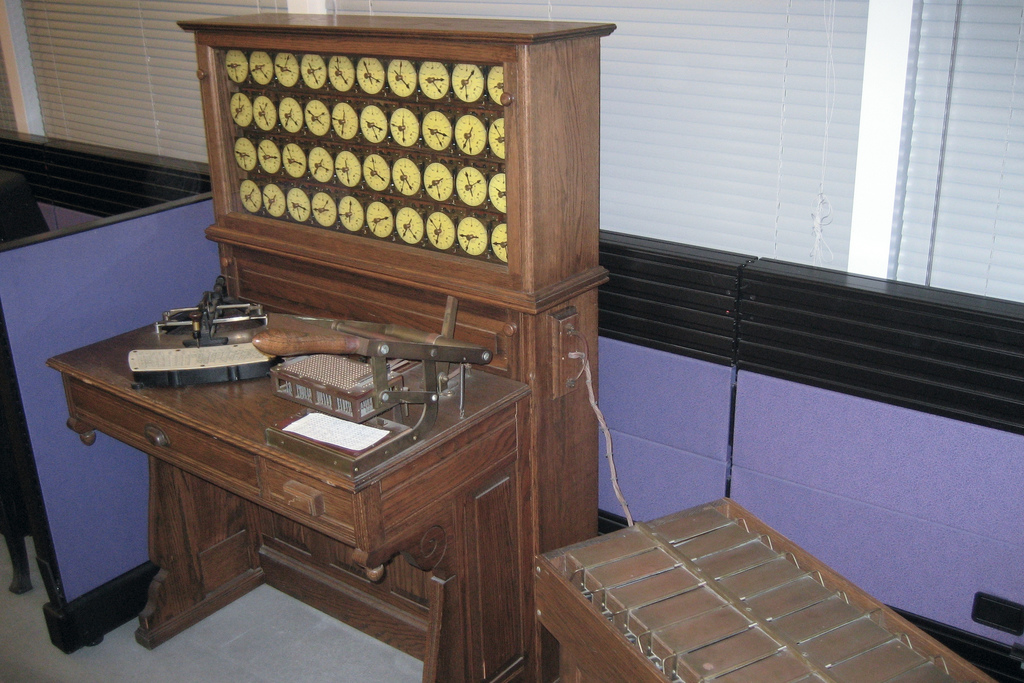
\includegraphics[width=\textwidth]{manuell}
  \caption{Tabelliermaschine von 1890 mit \enquote{pantograph punch}
    (\autoref{fig:pantograph}) links und Einlesevorrichtung rechts auf dem
    Schreibtisch. Oben die Zähler zu erkennen und rechts davon die
    Sortiermaschine~\cite{1890}.}
  \label{fig:1890}
\end{figure}

Hollerith hat für die Ausschreibung für die Volkszählung 1890 ein komplettes
System erarbeitet:

\begin{itemize}
  \item Die Daten wurden über eine Lochkartenstanze (\enquote{pantograph punch})
    eingegeben. Dabei wurde
    die Lochkarte in die Stanze oben eingelegt. Die verschiedenen Werte die
    eingegeben werden konnten, waren auf einer Vorlage mit Löchern unten in
    der Stanze notiert, so dass der Operator einen Hebel über die Vorlage
    bewegte und den Hebel in die betreffenden Löcher der Vorlage vertiefte.
    Dabei wurde gleichzeitig in die oben eingelegte Lochkarte das entsprechende
    Loch eingestanzt. Der Vorgang ist rein mechanisch. Die 1890 verwendeten
    Lochkarten waren unbedruckt, für das menschliche Ablesen der Karten
    lieferte Hollerith Vorlagen mit, die über die Lochkarten gelegt werden
    konnten~\cite{austrian1982herman}. \autoref{fig:pantograph} zeigt eine
    Stanze dieser Art, im Bild allerdings mit bedruckter Lochkarte. Das
    Prinzip ist in beiden Fällen das Gleiche.
  \item Die so gelochten Karten wurden in die Tabelliermaschine eingelesen,
    indem die Karte in die Lesevorrichtung eingelegt wurde und der Hebel dieser
    Vorrichtung nach unten gedrückt wurde. Dies führte dazu dass die Kontakte
    im Hebel durch die Löcher in der Lochkarte Schaltkreise schlossen die zum
    inkrementieren der jeweiligen, für die Löcher der Karte zugehörigen Werte
    führten. Die Tabelliermaschine selbst enthielt Reihen von Zähluhren, die
    diese Werte anzeigten und am Ende vom Operator abgelesen
    wurden~\cite{deutschesMuseum}.
  \item Nachdem die Karte eingelesen wurde, hat die Tabelliermaschine in der
    Sortiermaschine ein Fach geöffnet, in die die Lochkarte vom Operator
    reingelegt wurde.
\end{itemize}

Neben dem System von Hollerith wurden auch zwei weitere Systeme, von William C.
Hunt sowie Charles F. Pidgin, getestet. Als Testdaten wurde eine Untermenge der
tatsächlichen Daten des vorhergehenden Zensus von 1880 verwendet. Die
Untermenge enthielt Daten der Zählung von vier Auszählungsbezirken von St.
Louis und beschrieb 10.491 Einwohner. Getestet wurden \emph{Transkription}
(also das Aufnehmen der Daten in Lochkartenformat) sowie \emph{Verarbeitung}
(also das Tabellieren)~\cite{austrian1982herman}.

\begin{itemize}
  \item Hollerith-System: 72~Stunden, 27~Minuten für die Transkription sowie
    5~Stunden 28~Minuten für die Verarbeitung
  \item Hunt-System: 144~Stunden, 25~Minuten für Transkription, 55~Stunden,
    22~Minuten für Verarbeitung
  \item Pidgin-System: 110~Stunden, 56~Minuten für Transkription,
    44~Stunden, 41~Minuten für Verarbeitung
\end{itemize}

Aufgrund der deutlich schnelleren Arbeitsweise des Hollerith-Verfahrens,
insbesondere der Tabelliermaschine, war die Verwendung in der kommenden
Volkszählung beschlossen. Der Badarf an Tabelliermaschinen für die Zählung
wurde auf etwa 100 Stück geschätzt. Dabei wurden die Maschinen nicht an das
Büro verkauft, sondern gegen eine Gebühr verliehen. Diese Geschäftstaktik ist
darauf zurückzuführen, dass die Maschinen regelmäßiger und fachkundiger Wartung
bedürfen, für die Hollerith zuständig war. Hollerith war ebenfalls zuständig
für die notwendige Stromversorgung zu Sorgen, die 1890 noch nicht so
selbstverständlich war wie heutzutage~\cite{austrian1982herman}.

Zu dieser Zeit stellte Hollerith auch seinen ersten Angestellen an, Edmund
Talcott, den jüngeren Bruder von Lu Talcott, seiner zukünftigen Frau. Seine
Aufgaben bestanden darin, die Maschinen zusammenzusetzen, sie zu testen, die
Zähler zu verkabeln sowie die Maschinen für etwaige Reparaturen abzubauen.

Das System wurde im Zensusbüro aufgebaut und in Betrieb genommen. Die Karten
wurden verarbeitet und durch einen zweiten Durchlauf von einem anderen Operator
gegengeprüft, um menschliche Fehler auszuschließen. So konnte ein Bearbeiter
an einem Tag die Daten von bis zu 50.000 Personen verarbeiten, wie die
amerikanische Presse berichtete. Auch das Stanzen der Lochkarten war effizient.
Fähige Arbeiter steigerten sich von 500 Karten pro Tag auf 700 gestanzte Karten
täglich~\cite{austrian1982herman}.

Eine einzelne Lochkarte enthielt dabei 288~Positionen in 12~Reihen je
24~Löcher. Diese Löcher waren in \enquote{Felder} organisiert, welche alle
Antwortmöglichkeiten für das jeweilige Feld
repräsentierten~\cite{priestley2010science}.

Am 16.~August 1890 wurde die erste grobe Hochrechnung der Bevölkerung
fertiggestellt, nur sechs Wochen nach Beginn der Auswertung. Die offizielle
Zahl von 62.622.250 Einwohnern wurde jedoch erst am 12.~Dezember
verkündet~\cite{austrian1982herman}, da es einige Zeit dauerte, bis die
Ergebnisse aus allen Bundesstaaten der USA beim Zensusbüro ankamen.

Der Einsatz von Holleriths Maschinen führte zu massiven Zeitersparnissen.
Schätzungen gehen von etwa zwei Jahren aus, sowie von ungefähr 5~Millionen
Dollar\footnote{Entspricht inflationsbereinigt etwa 128~Millionen Dollar im
Jahr 2013} gesparten Steuergeldern. Somit kann man sagen, dass das System von Hollerith
sich erprobt hatte.

1892 verlegt Holleright sein Büro aus Washington nach Georgetown und gründet
dort die \enquote{The Tabulating Machine Company} (TMC).

% TODO: mehr?

\subsection{US-Volkszählung 1900}
\label{sec:1900}

Im Jahre 1900 war die Hälfte der Arbeitskräfte in den USA immer noch in der
Landwirtschaft tätig. Die Ernteausfälle 1894 führten zu starker
Unzufriedenheit, weshalb ein Ziel der Zählung im Jahr 1900 die Erfassung der
Landwirtschaftsstatistiken war. Damit sollte ein genauer Blick auf den Stand der
Landwirtschaft geworfen werden, was in früheren Jahren nicht möglich war.

Das Ziel dieser Statistik war es, Aussagen treffen zu können, ob große Farmen
produktiver arbeiten als kleinere Farmen, ob Pachtbauern genauso effizient sind wie
Bauern die ihr Land besitzen sowie ob Schwarze mehr Baumwolle auf ihren eigenen
oder gepachteten Feldern anbauen als Plantagen die von Weißen verwaltet
wurden\footnote{1900 wurde solch eine Aussage nicht direkt rassistisch
bewertet}.

Der Leiter des Zensus 1900, William R. Merriam, beauftragte am 18.~Mai 1899
eine Kommission \enquote{einen praktischen Test aller elektrischen
Buchhaltungsmaschinen oder Tabelliermaschinen oder anderer Maschinen, die
vorgeführt werden könnten}~\cite{austrian1982herman}. Wie sich herausstellte
kam Holleriths einzige Konkurrenz von Charles F. Pidgin, dessen Systeme er vor
zehn Jahren geschlagen hatte. Pidgin schickte drei Systeme ins Rennen, die
Evaluation mit Testdaten lieferte folgende Ergebnisse:

\begin{itemize}
  \item Hollerith-System: 185~Stunden, 53~Minuten
  \item Pidgin's Automatic Mechanical Tabulation System: 452~Stunden
  \item Pidgin's Electrical Typewriter Tabulator: nach 163~Stunden abgebrochen
  \item Pidgin's Pin Board System: Evaluation einvernehmlich gestoppt, da sehr
    ähnliche Effizienz zu Pidgins Electrical Typewriter Tabulator
\end{itemize}

Die Kommission stellte am 27.~Juli fest, dass sich keines der Konkurrenzsysteme
mit Holleriths System messen konnte.

Um die Anforderungen der Farmstatistiken zu erfüllen, war es notwendig, die in
den alten Maschinen verbauten Inkrementierer umzubauen. Im
Gegensatz zu den vorherigen Zählungen wo das Hochzählen von Werten ausgereicht
hat (etwa Personen in einem Haushalt, Anzahl der selbstständig Beschäftigten,
Immigranten aus Deutschland) war es für Farmen wichtig, die Größen der Felder
oder das Gewicht der jeweiligen Ernten zu addieren. Hollerith kannte die
Addierwerke von Tolbert Lanston, dem Erfinder der Monotype Satzmaschine und war
von diesen sehr angetan, weshalb die Erweiterung der Hollerith Maschinen kein
großes Problem war. Tatsächlich hatte Hollerith eine simple Variante davon bereits
1890 patentiert~\cite{truesdell1965development}.

\begin{figure}[h]
  \centering
  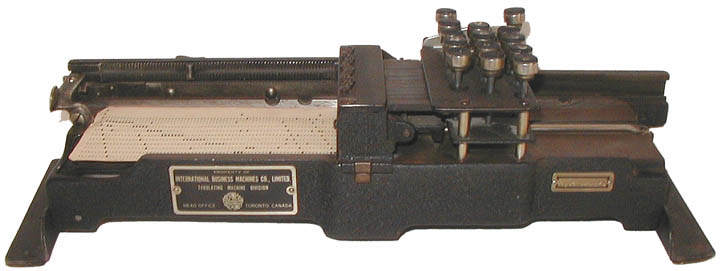
\includegraphics[width=\textwidth]{keypunch}
  \caption{Ein späteres Modell der \enquote{key punch}, man erkennt gut die
    Tasten und den Vorrückmechanismus~\cite{keypunch}}
  \label{fig:keypunch}
\end{figure}

Im Zuge der Modernisierung wurde auch eine neue Lochkartenstanze eingeführt,
die sogenannte \enquote{key punch}. Diese Stanze funktioniert ähnlich wie eine
Art einhändige Schreibmaschine in die die Lochkarte reingelegt wird und der
Operator die Daten über die Tasten eingibt. Dabei werden statt Typen auf Papier
löcher in die Karte gestanzt, mit automatischem Wagenlauf. Diese Art Lochstanze
war ein großer Erfolg und verblieb im wesentlichen unverändert 40~Jahre lang in
Verwendung.

Im Laufe der Auszählung wurde der Aufnahmemechanismus der Tabelliermaschinen
verbessert. Die Maschinen von 1890 wurden als \enquote{Hand}-Maschinen
bezeichnet, da der Operator die Karte von Hand in die Tabelliermaschine
einlegen musste. Hollerith verbesserte dieses System erstmals zu einem
\enquote{semi-automatic}-System, bei dem die Arbeit mit Elektromotoren
unterstützt wird. 1902 entwickelte er dieses weiter zum
\enquote{automatic}-System weiter, bei dem die gesamte Arbeit des Einlegens und
Einlesens automatisch abläuft: der Operator kann einen ganzen Stapel Karten in
die Maschine einlegen und diese zieht die unterste Karte vom Stapel ein,
tabelliert sie und gibt sie aus, so dass sie einsortiert werden
kann~\cite{austrian1982herman}. Da diese Maschinen erst spät perfektioniert
wurden, waren sie im eigentlichen Zensus von 1900 kaum im
Einsatz~\cite{truesdell1965development}.

Diese Verbesserung führte dazu, dass die automatischen Maschinen etwa sechsmal
so viel Arbeit verrichten konnten in der gleichen Zeit, also bis zu 415 Karten
pro Minute. An einem Tag konnten im Schnitt um die 90.000 Karten verarbeitet
werden\footnote{Die Maschine musste gestoppt werden um die Zähler abzulesen und
die Ergebnisse zu notieren}.

Aufgrund der erhöhten Verarbeitungsgeschwindigkeit führte das manuelle
Einsortieren der Karten zu Engpässen, daher musste ein Gerät entwickelt werden,
welches die Karten automatisch einsortieren kann. Holleriths Firma musste diese
Geräte im Einverfahren entwickeln, daher waren die 20~Geräte, die schließlich an
das Zensusbüro verkauft worden sind, eher krude. Nichtsdestotrotz wurde keine
spätere Zählung ohne die Hilfe von Sortiermaschinen
durchgeführt~\cite{truesdell1965development}.

\subsection{Kommerzielle Vermarktung}
\label{sec:commerce}

Die Tatsache, dass die Hollerith-Maschinen in den Volkszählungen genutzt worden
sind, war ein großer Triumph für Hollerith. Allerdings war die Vermietung der
Maschinen ein sehr wechselhaftes Geschäft, da die Maschinen zwischen den
jeweiligen Zählungen an TMC zurückgingen und keinen Umsatz brachten.
Holleriths Erstrebungen seine Technik auch im Ausland zu vermarkten, waren nur
teilweise erfolgreich. Zwar setzten Länder wie Norwegen sowie Kanada die
Maschinen erfolgreich ein, jedoch stieß der Einsatz der Maschinen in
Großbrittanien auf Sabotageakte durch Arbeiter, die um ihre Arbeit fürchteten.
In Österreich hingegen wurden seine österreichischen Patente aberkannt und die Maschinen
nachgebaut~\cite{austrian1982herman}.

Die erste Volkszählung Russlands, die von Zar Alexander III angeordnet wurde, war
eine beachtliche Gelegenheit für Hollerith, einen sehr großen Auftrag zu
bekommen. Jedoch bekam er bei der Ausschreibung Konkurrenz von den
Österreichern, die mit Holleriths eigener Technik in die Ausschreibung
einstiegen. Erst nach langwierigen Verhandlungen gelang es Hollerith am
12.~November 1896, die Ausschreibung für sich zu entscheiden~\cite{austrian1982herman}.

Ein weiteres Standbein musste her, um nicht vollständig von den Zensusbüros
abhängig zu sein. Hollerith erkannte dies schon frühzeitig, aber war mehr
Entwickler denn Geschäftsmann und konzentrierte sich lieber auf das Verbessern
der Maschinen als um kommerzielle Vermarktung. Nichtsdestotrotz waren die
ersten elektrischen Tabelliermaschinen von Hollerith 1887 im Gesundheitsministerium in Baltimore und in New Jersey im kommerziellen Einsatz sowie Mitte 1889 auch
in New York City~\cite{austrian1982herman}. Die Anschaffung dieser Systeme war
auf John Shaw Billings zurückzuführen, der, als Freund und Mentor Holleriths,
die Entwicklung der Maschinen durch Hollerith förderte.

Aufgrund früherer Erfahrungen im Eisenbahnunternehmen\footnote{Hollerith
arbeitete 1885 bis 1887 in einer Firma die Eisenbahn-Bremsen
herstellte~\cite{heide2009punched}, erfand dort auch elektrisch
ausgelöste Eisenbahn-Bremsen, die sich jedoch erst viele Jahre später
etablieren sollten~\cite{austrian1982herman}} war es für Hollerith
ersichtlich, dass die Eisenbahnunternehmen von seiner Erfindung profitieren
konnten. Holleriths erster Versuch in der Buchhaltung Fuß zu fassen, fand daher bei der
Eisenbahngesellschaft \enquote{New York Central} statt. 1895 wurden bei New York
Central 4~Millionen Frachtbriefe pro Jahr verarbeitet, woraufhin Hollerith
vorschlug, mithilfe von Lochkarten die Fracht sowie die Frachteinnahmen wöchentlich statt monatlich zu verarbeiten. Dies sollte das schnelle Bestimmen der profitablen Routen ermöglichen. Holleriths Argumente waren einleuchtend, so
dass er bereits im Herbst selbigen Jahres seine Maschinen in New York
aufstellte~\cite{austrian1982herman}. Im selben Jahr unternahm Hollerith zudem
eine Reise nach Russland, um die Verhandlungen für den dortigen Zensus zu führen,
woraufhin er bei seiner Rückkehr erfuhr, dass die Maschinen bei New York Central
außer Betrieb genommen wurden, da sie der Aufgabe nicht gewachsen seien.

Dieser Rückschlag führte dazu, dass Hollerith seine Maschinen wiederum
überarbeitete und die Zähluhren durch vier Addierer ersetzte, die vier
Bereichen der Lochkarten zugeordnet waren und vier Operationen gleichzeitig
ausführen konnten. Im Mai 1896 konnte Hollerith New York Central überzeugen,
einen weiteren Testlauf zu starten und konnte am 28.~September 1896 einen
Vertrag für den regulären Einsatz seiner Maschinen
unterzeichnen~\cite{austrian1982herman}. Hollerith legte seine Hoffnung darin, dass er, verweisend auf den Erfolg bei New York
Central, weitere Kunden gewinnen könnte. Jedoch dauerte es bis 1902, ehe er
kommerziellen Erfolg erzielen konnte.

Eine wichtige Entwicklung in dieser Hinsicht war die standarisierte Fertigung
von Waren. Früher war es üblich, dass jede Ware einzigartig angefertigt wurde.
So wurden Kleidergrößen erst im amerikanischen Bürgerkrieg standarisiert und immer mehr Ladenketten entwickelten Interesse daran, ihre Verkäufe zu analysieren. Für eine solche
Analyse waren Holleriths elektrische Tabelliermaschinen eine gute Wahl und so
setzte die Firma Marshall Field's sich mit Hollerith in Kontakt, um seine
Maschinen einzusetzen~\cite{austrian1982herman}. Zu dieser Zeit entschied sich Hollerith auch, die Maschinen nicht zu vermieten,
sondern sie kostenfrei zur Verfügung zu stellen, aber mit der Bedingung, dass die
Lochkarten bei TMC gekauft werden mussten. Damit hatte Hollerith eine Abrechnung nach
Bedarf eingeführt.

In den Jahren 1903 bis 1905 folgten viele Eisenbahnlinien schließlich dem
Vorbild der New York Central und begannen Experimente oder den Produktiveinsatz von
Holleriths System~\cite{austrian1982herman}. Um 1907 hatte sich das Kundennetz
so weit aufgespannt, dass es Schwierigkeiten gab, die Nachfrage nach Maschinen
zu erfüllen. Ein Problem, welches sich in das Jahr 1908 hin zog und erst Anfang
1909 gelöst wurde.

Es ist also ersichtlich: Holleriths Tabulating Machine Company konnte sich ein
zweites Standbein, den komerziellen Einsatz schaffen.

Im Jahre 1911 entschließt sich Hollerith schließlich seine Firma zu verkaufen
und TMC geht in einer neuen Firma, der \enquote{Computing Tabulating Recording
Company} (CTR) auf, die aus vier einzelnen Firmen
hervorgeht~\cite{austrian1982herman}:

\begin{enumerate}
  \item Computing Scale Company
  \item Tabulating Machine Company
  \item International Time Recording Company
  \item Bundy Manufacturing Company
\end{enumerate}

CTR wurde im Jahr 1924 wiederum in \enquote{International Business Machines
Corporation} (IBM) umbenannt, eine Firma die bis heute bekannt ist.

\section{Dehomag D11}
\label{sec:d11}

Eine konsequente Weiterentwicklung der Maschinen Holleriths war die Einführung
der D11 vom deutschen Unternehmen Dehomag, welche nach dem 2.~Weltkrieg in
IBM~450 umbennant wurde. Sie wurde 1932 bis 1936 von Hans Groß
entwickelt~\cite{deutschesMuseum}. Im Gegensatz zu Holleriths Maschinen für die
Volkszählungen wurde die D11 nun mit bedruckten Karten betrieben und hatte für
die Ausgabe einen Drucker, eine Innovation die Holleriths Konkurrenzfirma Powers als
Erstes eingeführt hatte~\cite{austrian1982herman}. Damit war es nicht mehr
nötig, die Verarbeitung zu stoppen, um die Ergebnisse zu sichern. Ein weiterer
Unterschied war, dass die D11 nicht nur die Addition, sondern ebenfalls
die Subtraktion beherrschte. Zudem war es möglich das Gerät optional mit
Multiplikation (bis zu 8 Stellen im Multiplikanden und 6 Stellen im
Multiplikator~\cite{rojas2002first}) sowie Division
auszustatten~\cite{deutschesMuseum}.

Die Entwicklung der D11 war zum einen Teil auf die deutsche Wirtschaftkrise im
Jahr 1929 und zum anderen Teil auf die Autarkiebemühungen der Nazis ab dem Jahr 1933
zurückzuführen. Frühere Tabelliermaschinen der Dehomag waren Importe aus den
USA, aber durch den 45\%-igen Rückgang der Importe wurde dieser Geschäftszweig
bedroht. Also baute die Dehomag 1933 ein Werk in Berlin, welches 1934 eröffnet
wurde. Ab 1935 wurde dort die D11 gebaut und bis 1943 wurden 1.120~Exemplare
hergestellt. Die Produktion endete erst im Jahr 1960~\cite{heide2009punched}.
In \autoref{fig:d11} ist das Exemplar der D11 zu sehen, welches im Deutschen
Museum ausgestellt ist, das Gerät ist funktionsfähig und kann in Betrieb
genommen werden\footnote{Stand 2013}. Man kann oben rechts die weißen
Lochkarten erkennen die zur Verarbeitung in die Maschine eingezogen werden. In
der Mitte befindet sich der Drucker, der Zwischenergebnisse ausgeben kann sowie
rechts die Sortierwerke. Auf der rechten Seite der Maschine befindet sich ein
Steckbrett, mit dem man die Verarbeitungsschritte durch umstecken ändern kann.
Das Steckbrett ist auch als ganzes austauschbar, was es ermöglicht mehrere
Programme zu \enquote{speichern} und das gerade benötigte Programm durch
einbauen zu \enquote{laden}, um nicht immer die Verbindungen umstecken zu
müssen.

\begin{figure}[h]
  \centering
  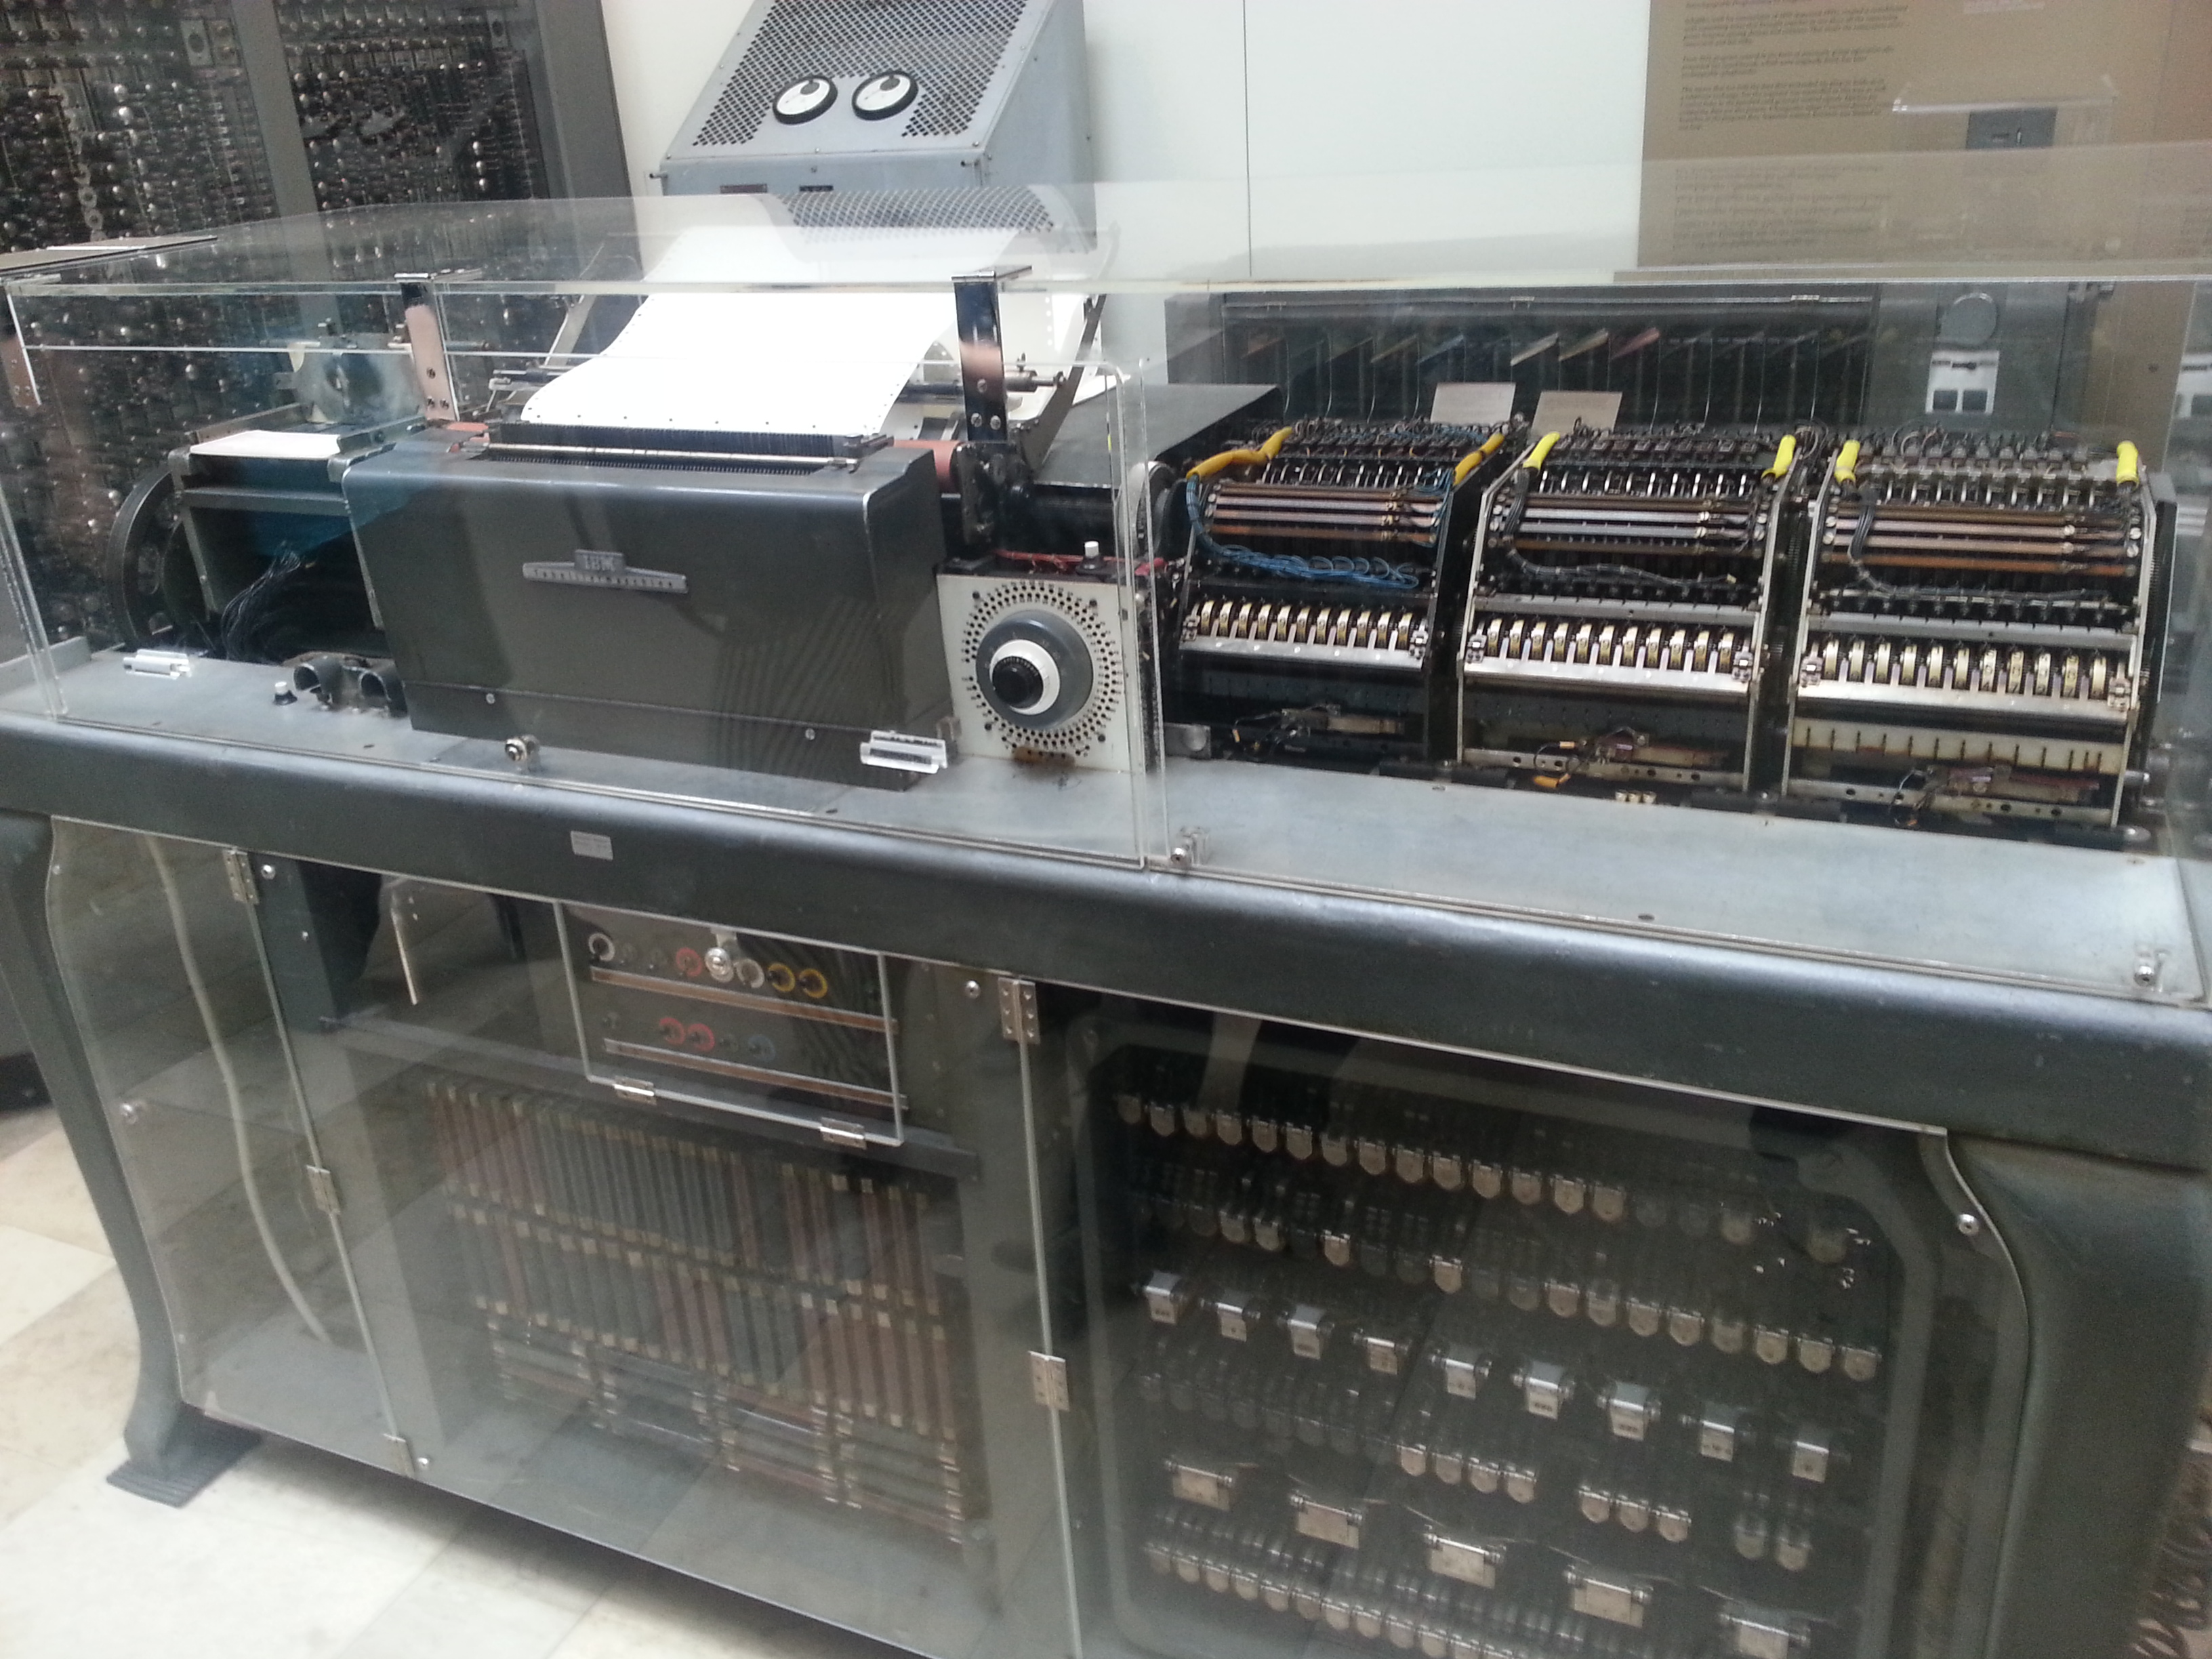
\includegraphics[width=\textwidth]{d11}
  \caption{Dehomag D11 im Deutschen Museum, im Hintergrund ist ebenfalls eine
    Sortiermaschine zu sehen, die in Kombination mit der D11 verwendet werden
    kann (eigene Aufnahme)}
  \label{fig:d11}
\end{figure}

\section{Eine deutsch-amerikanische Erfolgsgeschichte}

Wenn man sich über den Amerikaner Herman Hollerith und seine Erfindung die
Hollerith-Lochkarte informiert und welchen Einfluss diese Erfindung auf
Deutschland hatte, stößt man früher oder später auf die deutsche Firma
\enquote{Dehomag}. Die Firma tauchte bereits in einigen Ausführungen auf und In diesem Abschnitt soll der Werdegang der Dehomag nochmal genau erläutert
werden und weshalb sie bedeutend für die Entwicklung der Lochkartentechnik
ist.

\subsection{Anfangszeit der Dehomag}

Im November 1910 wurde die \enquote{Deutsche Hollerith-Maschinen Gesellschaft
mbH} oder kurz \enquote{Dehomag} von Willy Heidinger in Berlin
gegründet~\cite{dingwerth}. Das erste Werk hatte man in Villingen. Die Dehomag
produzierte Locher und Sortierer für die Hollerith-Lochkarten und
Tabelliermaschinen. Aufgrund der Inflation konnte die Dehomag während des
ersten Weltkrieges ihre Lizenzgebühren an die \enquote{Computing Tabulating
Recording Company} (CTR) nicht mehr bezahlen.  Daraufhin kaufte CTR 1922 90\%
der Firmenanteile der Dehomag auf~\cite{restloseErfassung}. 1924 wurde die CTR
übrigens in \enquote{International Business Machines Corporation} (IBM)
umbenannt. Nachdem das Werk in Villingen aufgelöst worden war, wurde ab 1927 in
Sindelfingen produziert. Im Januar 1934 wurde dann in
\enquote{Berlin-Lichterfelde mit über 400 Mitarbeitern ein eigenes
Produktionswerk sowie eine neue Hauptverwaltung}~\cite{dingwerth} der Dehomag
eröffnet.

\subsection{Von Dehomag zu IBM}

Nach der Erfindung der D11 konnte die Dehomag in den folgenden Jahren sowie
während des zweiten Weltkrieges Gewinne erwirtschaften. Allein in den ersten
acht Jahren wurden mehr als 1100 Tabelliermaschinen vom Typ D11
ausgeliefert~\cite{Kist95}. Das Wachstum der Dehomag in den Jahren 1935 bis 1942 
überstieg das Wachstum von Siemens im gleichen Zeitraum um
19\%~\cite{heide2009punched}. Ein Faktor, der die Verbreitung der D11 begünstigte, war die günstige politische
Lage der Firma Dehomag im Gegensatz zu ihrer Konkurrenz, vor allem dem
deutschen Ableger von Powers Firma. Die Dehomag wurde als deutsche Firma
gesehen, deren Maschinen in Deutschland entworfen und gebaut worden sind,
wohingegen Powers lediglich amerikanische Maschinen in Deutschland fertigte.
Willy Heidinger bestärkte diese \enquote{Deutschheit} der
Firma gegenüber den Nazis, indem er auf die deutschen Ursprünge der Lochkarten
und die deutsche Abstammung von Herman Hollerith, der als Deutsch-Amerikaner
bezeichnet wurde, hinwies und dessen Vorname dazu mit zwei \emph{n}, also
\emph{Hermann}, falsch buchstabiert wurde. Diese Bemühungen und der hohe
Bedarf an Tabelliermaschinen zahlten sich wie erwähnt finanziell und beim Wachstum aus. Die Dehomag trug somit entscheidend zur Verbreitung der
D11 in den Betrieben bei. Die Firma wurde stetig größer und 1940 war sie
bereits in Deutschland und Österreich in 59 Städten vertreten und beschäftigte
mehr als 2500 Mitarbeiter~\cite{dingwerth}. Wie beschrieben wurde 1960 schließlich die
letzte D11 gebaut und obwohl es die ersten programmierbaren Rechner gab, waren
zu der Zeit noch ungefähr 200 D11 Maschinen in Betrieb. Allerdings wurden die
D11 in den nächsten Jahren immer weniger genutzt und durch Computer ersetzt.
Heute steht eine der letzten restaurierten D11 Tabelliermaschinen in München im
Deutschen Museum~\cite{Kist95}.

Zu den Kunden der Dehomag gehörten unter anderem statistische Ämter, die
Industrie und während des Krieges die Wehrmacht sowie die Schutzstaffel der
Nationalsozialisten. Aufgrund des Krieges konnte IBM mit seiner Tochterfirma
Dehomag nur in neutralen oder von deutschen Truppen besetzten Ländern
zusammenarbeiten. Erst nach dem Ende des Krieges 1945 wurde IBM wieder in
Deutschland geschäftlich tätig. Im Jahr 1949 wurde die Dehomag dann in
\enquote{Internationale Büro-Maschinen Gesellschaft mbH} (IBM) umbenannt,
woraus später die \enquote{IBM Deutschland GmbH} wurde~\cite{sendler}.
Noch heute ist IBM in ganz Deutschland vertreten und gehört zu den führenden
Unternehmen im IT- Bereich. Es ist eine deutsch-amerikanische
Erfolgsgeschichte.

\section{Weiterentwicklung der D11}

Die Dehomag Tabelliermaschine D11 verkaufte sich wie erwähnt sehr gut, aber war
nicht die letzte Maschine in der Geschichte der Lochkartentechnik. Beim Einsatz
der D11 Maschine kristallisierten sich die Kritikpunkte eines unzureichenden
Zeichenvorrates, zu langsamer Druckgeschwindigkeit und zu geringer
arithmetischer Leistung heraus~\cite{sandner}. Im Jahr 1949 kam mit der
Buchungsmaschine IBM 407 eine Weiterentwicklung auf den Markt, die ein
neuartiges Druckwerk beinhaltete. Die Neuerung war ein sich nur vorwärts
drehendes, elektromagnetisch gesteuertes Rad. Dieses Rad wurde Typenrad genannt
und war der Träger des Zeichensatzes. Zusätzlich zum Alphabet und den
einstelligen Zahlen enthielt das Typenrad elf Sonderzeichen, welche nicht
chronologisch angeordnet waren (siehe \autoref{fig:typenrad}). Die Aufhängung
des Typenrades besorgte eine Schwinge, wodurch das Typenrad selbst zum Hammer
wurde. Mit dieser Technik konnte die Druckgeschwindigkeit erhöht und ein
qualitativ gutes Druckbild durch exakte Typenpositionierung gewährleistet
werden~\cite{sandner}. Ein weiterer Vorteil der IBM 407 war, dass die
Operationen auf den Lochkarten im Gegensatz zu vorher mit einem einzigen
Maschinenzyklus durchgeführt werden konnten~\cite{Boyell}. Aufgrund der
Möglichkeit der neuen Zeichenkombinationen wurden gleichzeitig neue
Kartenlocher und Prüfer entwickelt, damit die neue Technik eingesetzt werden
konnte.

\begin{figure}[h]
  \centering
  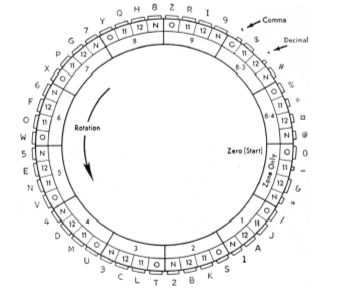
\includegraphics{typenrad}
  \caption{Schematisch dargestelltes Typenrad der IBM 407 von der Seite~\cite{sandner}}
  \label{fig:typenrad}
\end{figure}

Die Entwicklung und Produktion der IBM 407 fand bei IBM in der USA statt und
aufgrund der Währungsrelation war die Monatsmiete für eine IBM 407 in Europa
deutlich teurer als die Miete für ein Dehomag D11~\cite{sandner}. Aus diesem
Grund war die D11 in Europa verbreiteter. Anfang der 1950er Jahre kam mit der
Tabelliermaschine IBM 421 eine wichtige Weiterentwicklung für den europäischen
Markt heraus (siehe \autoref{fig:IBM421}). Diese besaß eine umfassende
Programmsteuerung und konnte an die gewünschten Arbeiten ihrer Anwender
angepasst werden~\cite{deutschesMuseum}. Sie besaß einen ähnlichen Zeichvorrat wie die IBM 407. Eine Alphabetzeile konnte ebenfalls
wie bei der IBM 407 in einem Maschinenzyklus gedruckt werden. Anstatt dem sich
vorwärts drehendem Typenrad wurde bei der IBM 421 wieder das
Typenstangendruckprinzip genutzt, wobei es für jede Typenstange eine neuartige
Antriebssteuerung gab. Durch das Einsetzen von mehreren Typenstangen konnte diese Maschine einen Mehrzeilendruck durchführen. Die Produktion der IBM 421 fand bei IBM Frankreich und
bei der in IBM Deutschland umbenannten Dehomag statt. \enquote{Aufgrund ihrer
Universalität war die 421 außer in Europa ein bis Nahost, Fernost, Afrika und
Südamerika gefragtes Produkt.}~\cite{sandner}.

\begin{figure}[h]
  \centering
  
\includegraphics{IBM421}
  \caption{Tabelliermaschine IBM 421~\cite{sandner}}
  \label{fig:IBM421}
\end{figure}

\section{Magnetische Speicherung ersetzt Lochkarte als Speichermedium}

Obwohl die IBM 421 in vielen Ländern zum Einsatz kam und \enquote{Anwender mit
um die 10 Tabelliermaschinen in der zentralen
Lochkartenabteilung}~\cite{sandner} keine Seltenheit waren, gehörte die IBM 421
zu den letzten Weiterentwicklungen. Der Grund dafür war die Verwendung der
magnetische Speicherung von binären Daten, wodurch die Lochkarten in den 1960er
Jahren als Medium für Massenspeicherung abgelöst wurden~\cite{gronau2009}. Bei
dieser Speichertechnik wird beim Schreiben eine Polaritätsänderung der
Ferritteile in der  ferromagnetischen Oberfläche erzeugt. Je nachdem, ob der
Bereich Richtung Nord- bzw. Südpol zeigt, wird beim Lesen die Richtung des
Magnetfeldes als 0 oder 1 interpretiert~\cite{gronau2009}. Für die magnetische
Speicherung können Bänder, Karten oder Platten genutzt werden. Das Prinzip der
Magnetspeicherung findet auch bei den heutigen Festplatten Anwendung.

Abschließend werden die Vor- und Nachteile dieser neuen Speichertechnik
genannt. Ein Vorteil von magnetischen Datenträgern gegenüber von Lochkarten ist
die Wiederverwendbarkeit. Alte Daten können gelöscht und neu überschrieben
werden. Außerdem sind die Kosten pro Gigabyte bei magnetischen Datenträgern
günstiger als bei den Lochkarten~\cite{Dee}. Aufgrund physikalischer und
technischer Grenzen hat der magnetisierte Bereich eine bestimmte Größe, weshalb
das Speichervolumen eines solchen Datenträger endlich ist. Ein Nachteil
magnetischer Datenträger ist somit, dass sie nicht beliebig klein sein können.

\section{Lochkarten im digitalen Zeitalter}

In diesem Abschnitt sollen Beispiele und Bereiche gezeigt werden, in denen auch
noch in dieser technisch weit vorangeschrittenen Zeit Lochkarten oder das
Prinzip der Lochkartentechnik zum Einsatz kommen. Die USA benutzt
beispielsweise vereinzelt in ihren Wahlautomaten Lochkarten, um ein schnelles
auswerten der Stimmen zu gewährleisten. So gaben bei der Präsidentschaftswahl
im Jahr 2000 die Bürger der Stadt Palm Beach im Bundesstaat Florida ihre Stimme
durch das Stanzen eines Loches in eine Lochkarte ab~\cite{simons}. Probleme bei
der Auswertung der Stimmen in Florida ließen die Lochkarten in Verruf geraten
und schließlich führte ein Urteil des Obersten Gerichtshof der Vereinigten
Staaten zum Wahlsieg von George W. Bush. Dennoch wurde bei der bisher letzten
US-Wahl 2012 \enquote{per Brief- oder Online-Wahl und - wie in manchen Gegenden
in Idaho - zum Teil auch noch mit Lochkarten}~\cite{keinVerfasser} abgestimmt.
Bei dieser Wahl gab es keine bekannten negative Zwischenfälle. Des Weiteren
existiert in der Stadt Conroe in Texas die Firma \enquote{Sparkler Filters},
die ihre Buchhaltungsaufgaben bis heute mit der Tabelliermaschine Sparklers IBM
402 auf Hollerith-Lochkarten ausführt~\cite{edwards}.

IBM benutzt zwar keine Tabelliermaschinen mehr, verwendet aber in seinem
Projekt \enquote{Millipede} das Grundprinzip der Lochkarten. Bei diesem Projekt
handelt es sich um eine Speichertechnik, welche im Nanometerbereich angewendet
wird.  Mit winzigen Messnadeln können Bits in einen Polymerfilm geschrieben,
gelesen oder gelöscht werden~\cite{binnig}. Eine Vertiefung im
Polymerfilm wird dabei als 1 und die unveränderte Oberfläche als 0
interpretiert. Der Unterschied zu herkömmlichen Lochkarten ist somit neben der
Größe die Möglichkeit Bits zu löschen und zu überschreiben. Mit dieser Technik
können bis zu ein Terabyte pro Quadratzoll (in²) gespeichert werden, wobei ein
Quadratzoll der Fläche von 6,4516cm² entspricht~\cite{binnig}. Die
Lese- und Schreibgeschwindigkeit kann durch Nutzung von mehreren parallel
arbeitenden Messnadeln optimiert werden.

Diese aufgezeigten Beispiele sind allerdings die Ausnahme, denn die
Lochkartentechnik ist in der heutigen Zeit veraltet und in der Computertechnik
nicht mehr von Bedeutung. Ein Zahlenbeispiel wird den technischen Fortschritt
im Bereich der Datenspeicherung belegen: Die am häufigsten verbreiteten
Lochkarten besaßen 80 Spalten und konnten somit 80 Byte speichern. Rechnet man
das auf eine 120 GB Festplatte hoch, so kommt man auf eine Anzahl von über 1,6
Milliarden Lochkarten, die die selbe Speicherkapazität wie diese Festplatte
besitzen~\cite{roeltgen}. Mittlerweile gibt es bereits Festplatten mit sehr
viel mehr als 120 GB Speicher.

\section{Fazit}

Der US-Amerikaner mit deutschen Wurzeln Herman Hollerith revolutionierte um 1900 die Datenverarbeitung. 
Inspiriert bei einer Fahrkartenkontrollen im Zug, ließ er Daten durch das Stanzen eines Loches auf einer 
Lochkarte festhalten. Außerdem baute er eine Maschine, die Tabelliermaschine, welche diese Daten dann nach ausgewählten Kriterien auswerten konnte. Diese mechanische 
Umsetzung der Auswertung von Daten konnte vorher nur per Hand durchgeführt werden. Dies vereinfachte und verkürzte 
die Arbeit beispielsweise bei Volkszählungen oder Buchhaltungsaufgaben.
Heutzutage ist die Lochkartentechnik veraltet und so gut wie nicht mehr im Einsatz. Die technische Entwicklung bis hin zur 
magnetischer Speicherung, welche die Lochkarte als Speichermedium ablöste, sowie Computer und Software haben diese Technik in der heutigen digitalen Welt ersetzt und vereinfacht.
Beispiele wie die Verwendung von Hollerith-Lochkarten für die Buchhaltungsaufgaben der Firma 
\enquote{Sparkler Filters} oder das Projekt \enquote{Millipede}, bei dem das Grundprinzip der Lochkartentechnik 
zum Speichern im Nanometerbereich verwendet wird, sind die Ausnahmen. Dennoch hat die Erfindung von Herman Hollerith 
über einen längeren Zeitraum die Arbeit der Menschen beeinflusst und ist ein wichtiger Bestandteil der Geschichte der Menschheit.


\printbibliography

\end{document}
